\section{Método de volumes finitos para equações hiperbólicas} % Seções são adicionadas para organizar sua apresentação em blocos discretos, todas as seções e subseções são automaticamente exibidas no índice como uma visão geral da apresentação, mas NÃO são exibidas como slides separados.

%----------------------------------------------------------------------------------------

\begin{frame}{Método de volumes finitos para equações hiperbólicas}
	Considerando uma lei de conservação hiperbólica da forma \eqref{EDPH}\ com $\phi = 1$ e $q = 0$, têm-se a forma unidimensional
	\begin{equation}\label{LeideConsevacaoMVF}
	  \frac{\partial c}{\partial t} + \frac{\partial}{\partial x}f(c) = 0.
	\end{equation}
	% Por simplicidade, a discretização será uniforme e centrada nos pontos: $x_i$, $i = 1,...,N$, de forma que as interfaces entre dois volumes de controle $V_{i-1}$ e $V_i$ são dadas por
	% \[
	%   x_{i\pm \frac{1}{2}} = x_i \pm \frac{\Delta x}{2}.
	% \]
	% Com isso, cada volume de controle é dado por
	% \[
	%   V_i = [x_{i-\frac{1}{2}},x_{i+\frac{1}{2}}).
	% \]
	% A discretização temporal também será considerada uniforme, com cada passo de tempo de tamanho $\Delta t$, sendo cada nível denotado por $t^n = n\Delta t$.
	Em cada $t^n$, definine-se:
	\[
	  C_i^n = \frac{1}{\Delta x}\int_{x_{i-\frac{1}{2}}}^{x_{i+\frac{1}{2}}}c(x,t^n)\ dx \quad \text{ e } \quad
		\bar{F}_{i\pm\frac{1}{2}}^n = \frac{1}{\Delta t}\int_{t^n}^{t^{n+1}}f(c(x_{i\pm\frac{1}{2}},t))\ dt.
	\]
	Integrando a lei de conservação \eqref{LeideConsevacaoMVF} em $[x_{i-\frac{1}{2}},x_{i+\frac{1}{2}}) \times [t^n,t^{n+1})$, separando as integrais e utilizando o teorema fundamental do cálculo, têm-se:
	\begin{equation}\label{eqDaConcentracao}
	  C_i^{n+1} = C_i^n - \frac{\Delta t}{\Delta x}\left(\bar{F}_{i+\frac{1}{2}}^n - \bar{F}_{i-\frac{1}{2}}^n\right).
	\end{equation}
	Ou seja, a equação acima estabelece um princípio de conservação: \textit{a variação média da concentração na célula é dada pela diferença dos fluxos nas fronteiras da mesma}; ainda sem quaisquer tipos de aproximações.
\end{frame}

%----------------------------------------------------------------------------------------

% \begin{frame}{Método de volumes finitos para equações hiperbólicas}
% 	A representação pode ser dada por uma malha tal como:
% 	\begin{figure}[H]
% 	\centering
% 	\begin{tikzpicture}[scale=1]
% 	  \draw[black] (-0.3,-1.0) -- (3.3,-1.0);
% 	  \draw[black] (-0.3, 0.0) -- (3.3, 0.0);
% 	  \draw[black] (-0.3, 1.0) -- (3.3, 1.0);

% 	  \draw[black] (0.0,-1.3) -- (0.0,1.3);
% 	  \draw[black] (1.0,-1.3) -- (1.0,1.3);
% 	  \draw[black] (2.0,-1.3) -- (2.0,1.3);
% 	  \draw[black] (3.0,-1.3) -- (3.0,1.3);

% 	  \draw[black] (1.0,-1.3) node[below] {${x_{i-1/2}}$};
% 	  \draw[black] (2.0,-1.3) node[below] {${x_{i+1/2}}$};
% 	  \draw[black] (3.3,-1.0) node[right] {${t^{n}}$};
% 	  \draw[black] (3.3, 0.0) node[right] {${t^{n+1}}$};

% 	  \draw[black] (0.5,-0.5) node {$\mathbf{C_{i-1}^{n}}$};
% 	  \draw[black] (1.5,-0.5) node {$\mathbf{C_{i}^{n}}$};
% 	  \draw[black] (2.5,-0.5) node {$\mathbf{C_{i+1}^{n}}$};
% 	  \draw[black] (1.5, 0.5) node {$\mathbf{C_{i}^{n+1}}$};
% 	\end{tikzpicture}
% 	%\caption{Representação da malha.}
% 	\label{fig:discrLCH}
% 	\end{figure}
% 	Em cada $t^n$, a aproximação da solução no volume de controle é dada pelo valor médio de concentração nessa célula:
% 	\[
% 	  C_i^n = \frac{1}{\Delta x}\int_{x_{i-\frac{1}{2}}}^{x_{i+\frac{1}{2}}}c(x,t^n)\ dx,
% 	\]
% 	e também, define-se uma média temporal da função fluxo
% 	\[
% 	  \bar{F}_{i\pm\frac{1}{2}}^n = \frac{1}{\Delta t}\int_{t^n}^{t^{n+1}}f(c(x_{i\pm\frac{1}{2}},t))\ dt.
% 	\]
% \end{frame}

%----------------------------------------------------------------------------------------

% \begin{frame}{Método de volumes finitos para equações hiperbólicas}
% 	Integrando a lei de conservação \eqref{LeideConsevacaoMVF} em $[x_{i-\frac{1}{2}},x_{i+\frac{1}{2}}) \times [t^n,t^{n+1})$:
% 	\[
% 	  \int_{t^n}^{t^{n+1}}\int_{x_{i-\frac{1}{2}}}^{x_{i+\frac{1}{2}}}\left(\frac{\partial c}{\partial t} + \frac{\partial}{\partial x}f(c)\right)\ dx\ dt = 0,
% 	\]
% 	separando as integrais e utilizando o teorema fundamental do cálculo, têm-se:
% 	\begin{equation}\label{eqDaConcentracao}
% 	  C_i^{n+1} = C_i^n - \frac{\Delta t}{\Delta x}\left(\bar{F}_{i+\frac{1}{2}}^n - \bar{F}_{i-\frac{1}{2}}^n\right).
% 	\end{equation}
% 	Ou seja, a equação acima estabelece um princípio de conservação: \textit{a variação média da concentração na célula é dada pela diferença dos fluxos nas fronteiras da mesma}; ainda sem quaisquer tipos de aproximações.
% \end{frame}

%----------------------------------------------------------------------------------------

\begin{frame}{Método upwind para aproximação de fluxos discretos}
	Para aproximar os fluxos discretos $F^n_{i\pm 1/2}$, pode-se usar diversos métodos, como:
	\begin{itemize}
		\item \textit{Esquema central} (diferenças finitas);
		\item Método de \textit{Lax-Friedrichs}; ou
		\item Método de \textit{Lax-Wendroff}.
	\end{itemize}

	O método usado neste trabalho será o \textbf{método upwind}, que leva em conta a \textit{estrutura da solução}, de modo que a informação em cada ponto é obtida olhando a direção na qual a mesma se propaga.
		\begin{figure}[H]
	\centering
	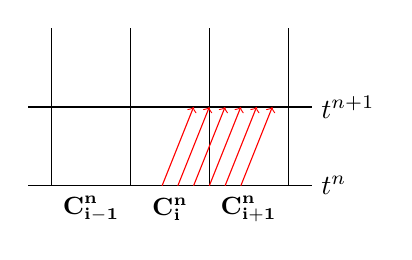
\begin{tikzpicture}[scale=1]
	  \draw[black] (-0.3,-1.0) -- (3.3,-1.0);
	  \draw[black] (-0.3, 0.0) -- (3.3, 0.0);

	  \draw[black] (0.0,-1) -- (0.0,1);
	  \draw[black] (1.0,-1) -- (1.0,1);
	  \draw[black] (2.0,-1) -- (2.0,1);
	  \draw[black] (3.0,-1) -- (3.0,1);

	  \draw[black] (3.3,-1.0) node[right] {${t^{n}}$};
	  \draw[black] (3.3, 0.0) node[right] {${t^{n+1}}$};

	  \draw[black, font=\small] (0.5,-1.3) node {$\mathbf{C_{i-1}^{n}}$};
	  \draw[black, font=\small] (1.5,-1.3) node {$\mathbf{C_{i}^{n}}$};
	  \draw[black, font=\small] (2.5,-1.3) node {$\mathbf{C_{i+1}^{n}}$};
		
		\foreach \x in {1.0,1.2,1.4,1.6,1.8,2.0} {
	    \draw[->, red] (\x+.4,-1.0) -- (\x+.8,0.0);
	  }
	\end{tikzpicture}
	\caption{Propagação da informação em uma célula.}
	\label{fig:discrLCH}
	\end{figure}
\end{frame}

%----------------------------------------------------------------------------------------

\begin{frame}{Método upwind: Caso unidimensional}
	Considerando $u^+ = \text{max}\{u,0\}$ e $u^- = \text{min}\{u,0\}$, é possível discretizar \eqref{eqDaConcentracao} no caso de \textbf{velocidades constantes}:
	\begin{equation}\label{eqUWVelConstante}
	  \begin{aligned}
	    C_i^{n+1} &= C_i^n - \frac{\Delta t}{\Delta x}\left(u^+C^n_{i} + u^-C^n_{i+1} - u^+C^n_{i-1} - u^-C^n_{i}\right).
	  \end{aligned}
	\end{equation}
	Agora, no caso de \textbf{velocidades variáveis}:
	\begin{equation}\label{eqUWVelVariadas}
		\begin{aligned}
		C_i^{n+1} &= C_i^n - \frac{\Delta t}{\Delta x} \left[ \left( u^+(x_{i+\frac{1}{2}}) - u^+(x_{i-\frac{1}{2}}) + u^-(x_{i+\frac{1}{2}}) - u^-(x_{i-\frac{1}{2}}) \right) C_i^n \right] \\
		&- \frac{\Delta t}{\Delta x} \left[ u^-(x_{i-\frac{1}{2}}) W_{i-\frac{1}{2}} + u^+(x_{i+\frac{1}{2}}) W_{i+\frac{1}{2}} \right].
		\end{aligned}
	\end{equation}
	Também, é preciso satisfazer a \textbf{condição CFL}, uma condição necessária, mas não suficiente, para garantir convergência do método de volumes finitos para a equação diferencial. A convergência ocorre caso:
	\[
	  u\frac{\Delta t}{\Delta x} \leq 1,
	\]
	com $u$ constante.
\end{frame}

%----------------------------------------------------------------------------------------

\begin{frame}{Método upwind: Exemplo do caso unidimensional}
	\begin{exemplo}
		\justifying
		Dado o problema de contorno unidimensional \eqref{escoamento_base}, que modela o escoamente monofásico de um reservatório saturado, com sistema de equações dado por:
	  \begin{equation}\label{Elip282}
	    \left\{
	      \begin{aligned}
	      -\frac{d}{dx}\left(K\frac{dp}{dx}\right) &= -25\cos(25x) && \text{em $\Omega_e = [0,1]$} \\
	      p &= x && \text{sobre $\partial\Omega_e$}
	      \end{aligned}
	    \right.
	  \end{equation}
	  onde $K(x) = 2 + \sin(25x)$. Será simulado o fluxo de um contaminante com concentrações $c(x,t)$, governado pelo sistema:
	  \[
	  \left\{
	    \begin{aligned}
	      \partial_t c + u\partial_xc &= 0 && \text{em $\Omega_h$} \\
	      c_0(x) &= e^{-20(3x-.5)^2} + e^{-(3x-3.5)^2}&& \text{em $\Omega_h$}
	    \end{aligned}
	  \right.,
	  \]
	  Utilizando a equação \eqref{eqUWVelVariadas}, é possível chegar numa solução visualizada pelos gráficos a seguir:
	\end{exemplo}
\end{frame}

%----------------------------------------------------------------------------------------

\begin{frame}{Método upwind: Exemplo do caso unidimensional}
	\begin{exemplo}
		\centering
	  \animategraphics[autoplay,loop,width=0.8\linewidth]{30}{1dVFUW_frames_temp/frame_}{000}{100}
	\end{exemplo}
\end{frame}

%----------------------------------------------------------------------------------------

\begin{frame}{Método upwind: Caso bidimensional}
	Para problemas em duas dimensões, a lei de conservação \eqref{LeideConsevacaoMVF} assume a forma
	\begin{equation}\label{LC2D}
	  c_t + f_x(c) + g_y(c) = 0,
	\end{equation}
	onde a concentração do fluido depende de $x$, $y$ e $t$. Definindo
	\begin{equation}
	  \bar{F}_{i+\frac{1}{2},j}^{n} = \frac{1}{\Delta t \Delta y} \int_{t^{n}}^{t^{n+1}} \int_{y_{j-\frac{1}{2}}}^{y_{j+\frac{1}{2}}} f(c(x_{i+\frac{1}{2}}, y, t)) \, dy \, dt
	\end{equation}
	e
	\begin{equation}
	  \bar{G}_{i,j+\frac{1}{2}}^{n} = \frac{1}{\Delta t \Delta x} \int_{t^{n}}^{t^{n+1}} \int_{x_{i-\frac{1}{2}}}^{x_{i+\frac{1}{2}}} g(c(x, y_{j+\frac{1}{2}}, t)) \, dx \, dt,
	\end{equation}
	têm-se
	\begin{equation}
	  C_{i,j}^{n+1} = C_{i,j}^{n} - \frac{\Delta t}{\Delta x} \left( \bar{F}_{i+\frac{1}{2},j}^{n} - \bar{F}_{i-\frac{1}{2},j}^{n} \right) - \frac{\Delta t}{\Delta y} \left( \bar{G}_{i,j+\frac{1}{2}}^{n} - \bar{G}_{i,j-\frac{1}{2}}^{n} \right)
	\end{equation}
	onde os fluxos $\bar{F}$ e $\bar{G}$ podem ser aproximados por fluxos discretos em cada direção, assim como em \eqref{eqUWVelConstante}\ ou \eqref{eqUWVelVariadas}.
\end{frame}

%----------------------------------------------------------------------------------------

\begin{frame}{Método upwind: Exemplo do caso bidimensional}
	\begin{exemplo}\label{ex2CB}
		O primeiro exemplo é o mais simples: um problema elíptico bidimensional simplificado como \eqref{escoamento_base}, uma configuração \textit{a quarter of the five spot} como na definição \ref{qot5} e condições de contorno homogêneas de Neumann:
	  \[
	    \left\{
	      \begin{aligned}
	      \nabla \cdot u &= q && \text{em $\Omega = [0,1]\times [0,1]$} \\
	      u\cdot n &= 0 && \text{sobre $\partial\Omega$} \\
	      -K \nabla p &= u && \text{(Velocidade de Darcy)}
	      \end{aligned}
	    \right..
	  \] 
	  Com uma permeabilidade absoluta $K(x,y) = 1$ constante, termo fonte $\tilde{q} = 1$, poço de injeção na célula $(1,1)$ e poço de produção em $(N,M)$.
	\end{exemplo}
\end{frame}

%----------------------------------------------------------------------------------------

\begin{frame}
	\begin{exemplo}
		\centering
	  \animategraphics[autoplay,loop,width=0.75\linewidth]{30}{1ex2dVFUW_frames_temp/frame_}{0000}{0100}
	\end{exemplo}
\end{frame}

%----------------------------------------------------------------------------------------
\begin{frame}{Método upwind: Exemplo do caso bidimensional}
	\begin{exemplo}\label{ex2CB}
		\justifying
	  Neste segundo exemplo, dado um problema elíptico bidimensional simplificado como \eqref{escoamento_base}, uma configuração \textit{a quarter of the five spot}, campo de permeabilidade e de pressões e velocidades visualizados abaixo:
	  \begin{figure}[H]
	    \centering
	    \begin{subfigure}[c]{0.4\textwidth}
	      \centering
	      \includegraphics[width=\textwidth]{img/ex2_perm_hetero.png}
	    \end{subfigure}
	    \begin{subfigure}[c]{0.4\textwidth}
	      \centering
	      \includegraphics[width=\textwidth]{img/ex2_pressao_velocidade.png}
	    \end{subfigure}
	    \caption{Gráficos de permeabilidade e de pressão com velocidades não normalizadas.}
	  \end{figure}
	\end{exemplo}
\end{frame}

%----------------------------------------------------------------------------------------

\begin{frame}
	\begin{exemplo}
		\centering
	  \animategraphics[autoplay,loop,width=0.75\linewidth]{30}{2ex2dVFUW_frames_temp/frame_}{0000}{0100}
	\end{exemplo}
\end{frame}

%----------------------------------------------------------------------------------------